\chapterimage{Water1.png} % Chapter heading image
\chapter{Regulations}
\section{Regulations Related to Wastewater Treatment}\index{Regulations Related to Wastewater Treatment}
This is for establishing the level of treatment of the wastewater.
\subsection{Treated Wastewater - NPDES Permit}\index{Treated Wastewater - NPDES Permit}
The National Pollutant Discharge Elimination System (NPDES) permit program program addresses water pollution by regulating point sources that discharge pollutants to waters of the United States.

\begin{itemize}
\item The NPDES permit program was created in 1972 by the Clean Water Act (CWA).
\item Applies to sources that discharge pollutants to waters of the United States.
\item Requires all facilities discharging “pollutants” into any body of water in the USA to obtain and comply with a \hl{NPDES permit}.
\item NPDES permit \hl{establishes} \textul{discharge limits}, \textul{monitoring} and \textul{reporting} \hl{requirements}\\
\item In California, the responsibility of implementing the federal NPDES program is delegated to the State of California through the State Water Resources Control Board (State Water Board or SWRCB) and the nine Regional Water Quality Control Boards (Regional Water Boards), collectively Water Boards. In California, NPDES permits are also referred to as waste discharge requirements (WDRs) that regulate discharges to waters of the United States.
\end{itemize}

\section{Sewage Sludge/Biosolids Regulations}\index{Sewage Sludge/Biosolids Regulations}
The Clean Water Act also stipulates control of the the quality of sludge/biosolids produced from the wastewater treatment operations.  Federal Regulation 40CFR Part 503 also known as Rule 503  as stipulated by the Clean Water Act 
			\begin{itemize}
				\item Part 503 rule applies to any person who applies biosolids to the land or fires biosolids in a biosolids incinerator, and to the owner/operator of a surface disposal site, or to any person who is a preparer or generator of biosolids for use, incineration, or disposal.
				\item Part 503 standard includes:
					\begin{enumerate}
						\item General requirements
						\item Pollutant limits
						\item Management practices
						\item Operational standards, and
						\item Requirements for the frequency of monitoring, record-keeping, and reporting
					\end{enumerate}
			\end{itemize}

\section{Air Quality Regulations}\index{Air Quality Regulations}
\begin{itemize}
\item Air emissions from wastewater collections and treatment systems are subject to federal, state and local air quality related rules and regulations established to protect human health and comfort, and the environment.  
\item Typically, a local agency such as the South Coast Air Quality Management District is designated to enact and enforce air quality rules and regulations which apply to all sources of air emissions including wastewater treatment plants.
  
\item Related to its air pollutants emissions, Wastewater treatment plants are required to:
\begin{itemize}
\item Obtain air quality related operating permits for equipment and processes which emit air pollutants and for its systems treating foul air.
\item Implement air emission pollutants control measures
\item Comply with record keeping and reporting requirements
\item Comply with air quality rules to prevent public nuisance and protect public health and safety
\end{itemize}

also include ones to protect Many states As in other states, California Health and Safety Code Section 41700 and District Rule 51 states that no person can discharge air contaminants that cause injury, nuisance or annoyance to any considerable number of persons or the public, or that endanger the comfort, health or safety of such persons.

\end{itemize}

\section{Regulations Related to Operations and Maintenance}\index{Regulations Related to Wastewater Treatment Operations and Maintenance}
\subsection{Operator Certification}\index{Operator Certification}
\begin{itemize}
\item The requirements of the Operator Certification program is established for each state.  These meet the Operator Certification Requirements of the regulations stemming from the 1996 Amendments to the Safe Drinking Water Act.
\item The goal is to ensure that operators of wastewater treatment facilities in the State meet the minimum level of competence; thereby, protecting public health and the environment.
\item In California, the Wastewater Operator Certification program (WWOCP) administers Wastewater Treatment Plant Certification examinations, certifications (grades I to V), and certification renewals. 
\item WWOCP classifies Wastewater Treatment Plants and stipulates that no person shall operate a wastewater treatment plant unless that person has been certified by the division as a wastewater treatment plant operator or operator-in-training at a grade appropriate for the class of plant being operated.
\item A certified operator or operator-in-training may be subject to administrative sanctions including reprimand or denial, suspension, probation, or revocation of the operator certification for performing, or allowing or causing another to perform acts which include:
\begin{itemize}
\item Operating or allowing the operation of a wastewater treatment plant by a person who is not certified at the grade necessary for the position
\item failing to use care or good judgment in the course of employment as an operator or failing to apply knowledge or ability in the performance of duties.
\item Negligence causing the violation of appropriate waste discharge requirements of the NPDES permit
\end{itemize}
\end{itemize}
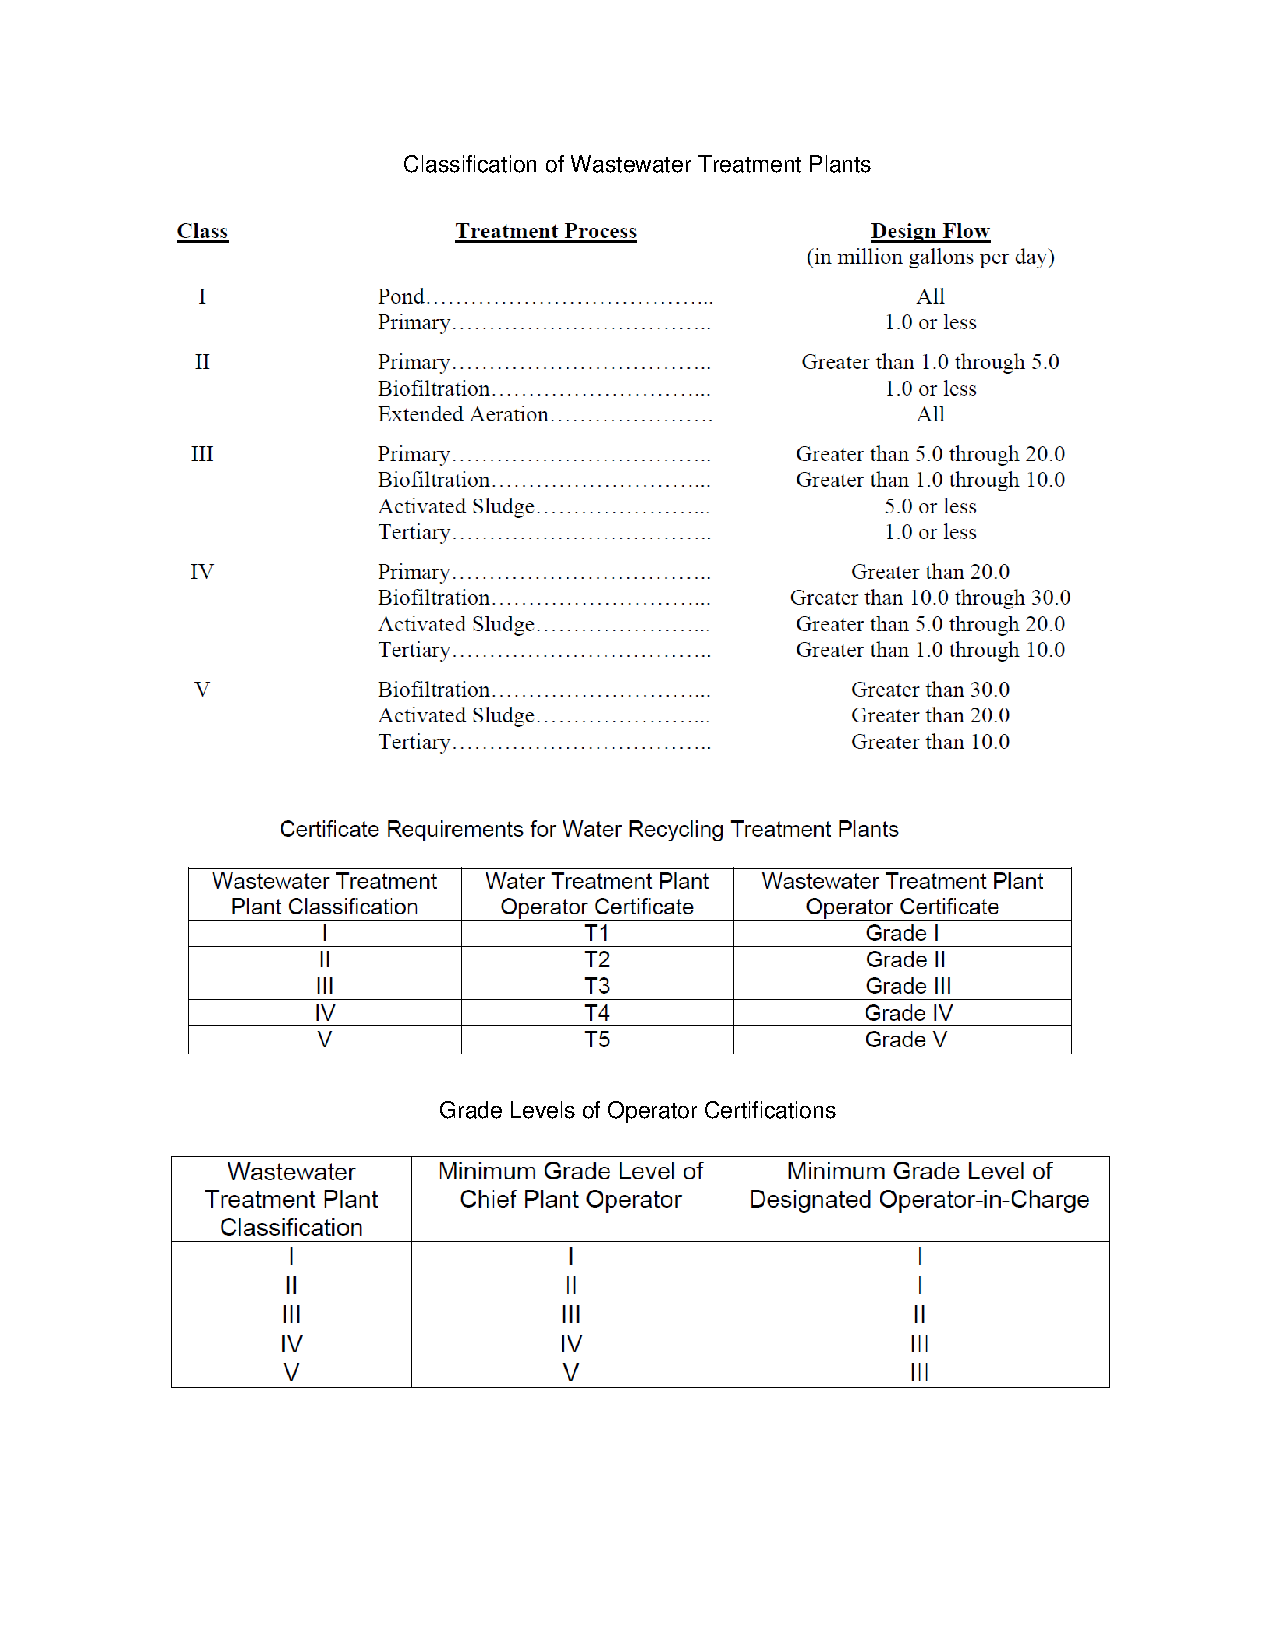
\includepdf[pages=-]{WastewaterPlantOperatorClassificationRequirements.pdf}
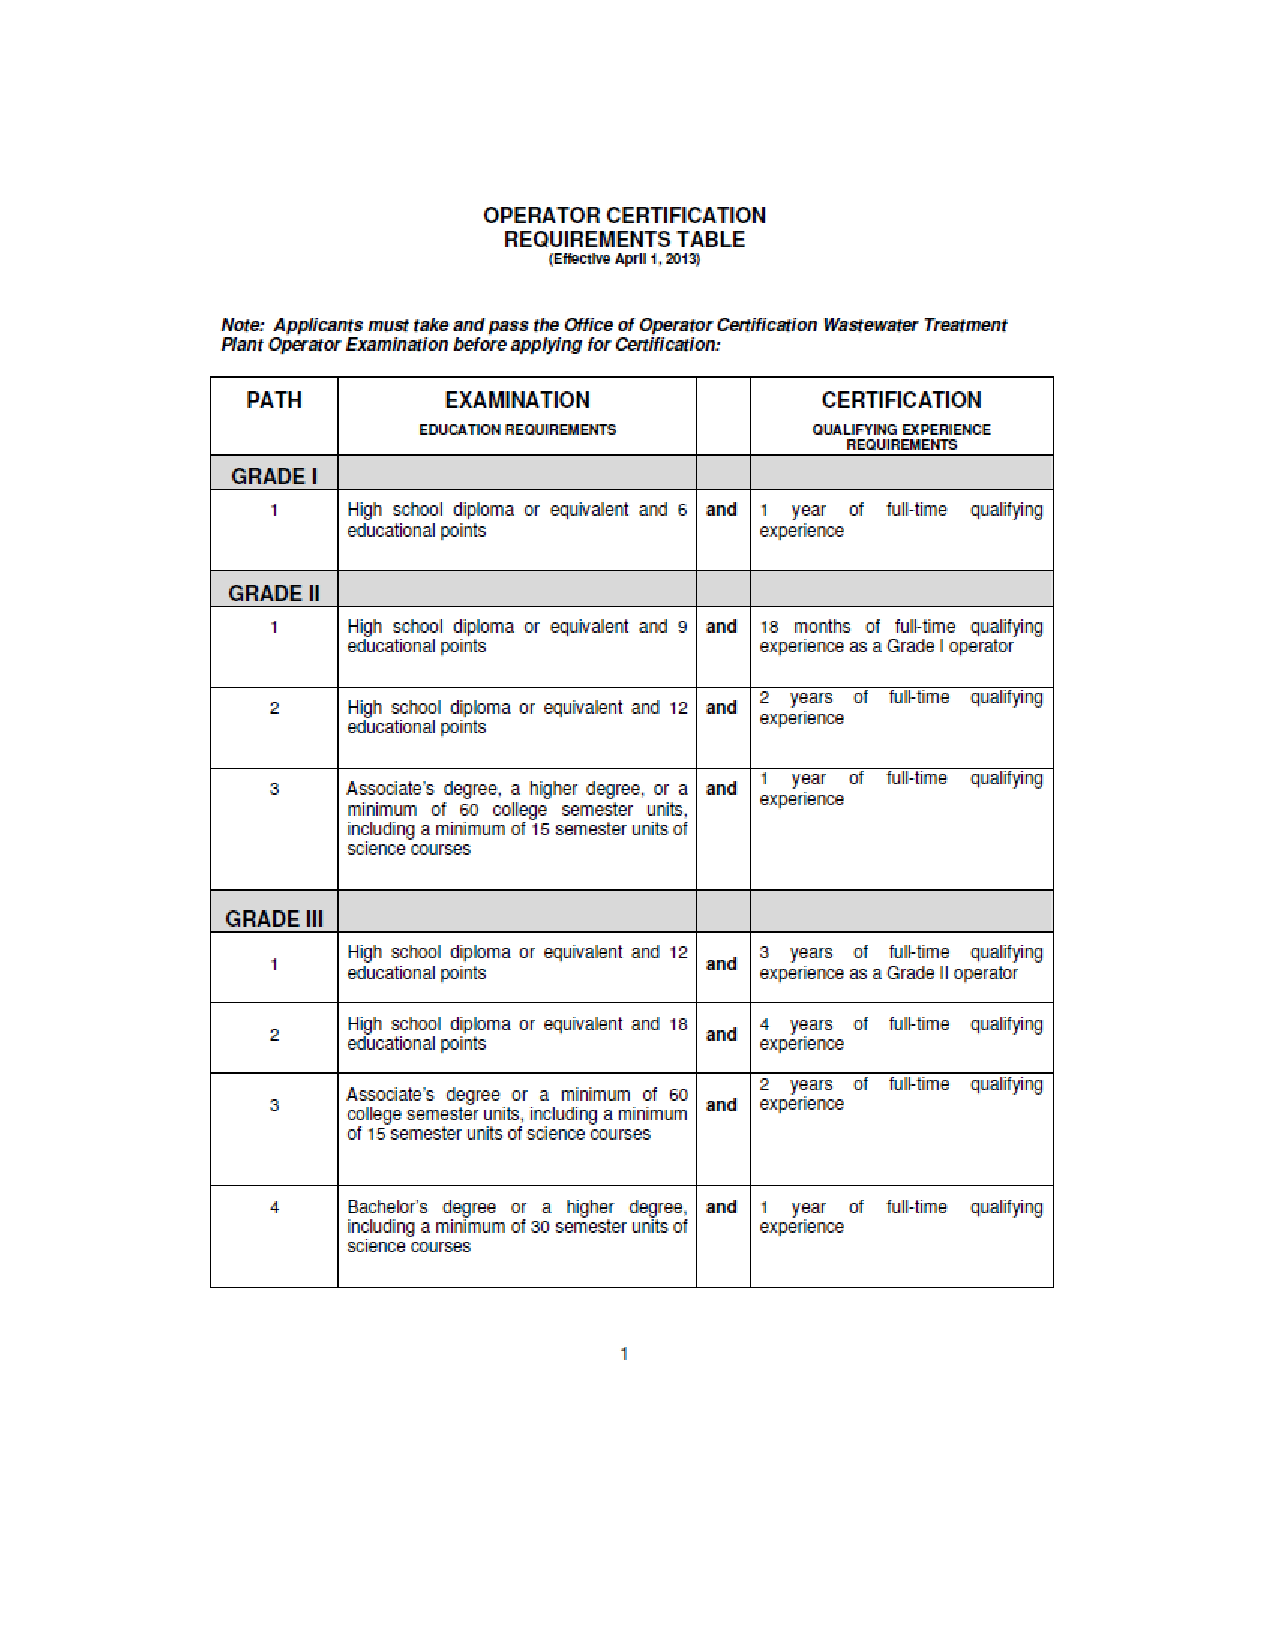
\includepdf[pages=-]{CertificationRequirement.pdf}

\subsection{Worker Safety}\index{Worker Safety}
\begin{itemize}
\item Wastewater treatment facility can be an extremely unsafe occupational field
\item It involves most of the major categories of workplace hazards:  biological, chemical, physical, safety and ergonomic,  accentuated with other factors such as shift work and diverse tasks.
\item Entities including The Occupational Safety and Health Administration(OSHA) National Electrical Code (NEC), National Fire Protection Association (NFPA), Underwriters Laboratory (UL) have recognized these hazards and implemented codes and standards to protect the affected persons and wastewater workers.
\end{itemize}
\end{document}